\begin{figure}[t]
\centering
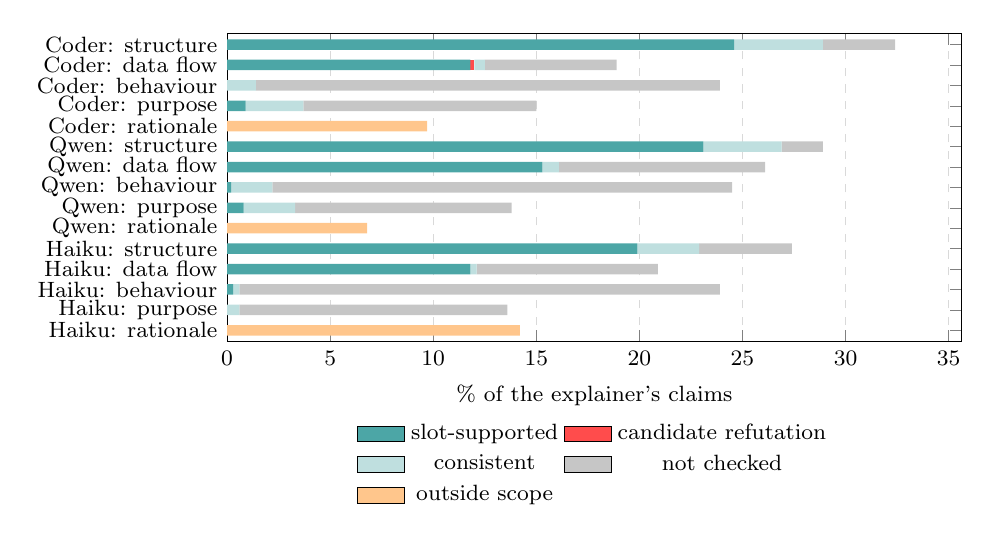
\begin{tikzpicture}
\begin{axis}[xbar stacked, width=0.90\columnwidth, height=5.5cm, bar width=3.8pt, xmin=0, xlabel={\% of the explainer's claims}, symbolic y coords={Haiku: rationale,Haiku: purpose,Haiku: behaviour,Haiku: data flow,Haiku: structure,Qwen: rationale,Qwen: purpose,Qwen: behaviour,Qwen: data flow,Qwen: structure,Coder: rationale,Coder: purpose,Coder: behaviour,Coder: data flow,Coder: structure}, ytick=data, yticklabel style={font=\footnotesize}, xticklabel style={font=\footnotesize}, label style={font=\footnotesize}, legend style={font=\footnotesize, at={(0.5,-0.23)}, anchor=north, legend columns=2, draw=none}, xmajorgrids, grid style={dashed,gray!30}, enlarge y limits=0.04]
\addplot[xbar,draw=none,fill=teal!70,area legend] coordinates {(24.6,Coder: structure) (11.8,Coder: data flow) (0.0,Coder: behaviour) (0.9,Coder: purpose) (0.0,Coder: rationale) (23.1,Qwen: structure) (15.3,Qwen: data flow) (0.2,Qwen: behaviour) (0.8,Qwen: purpose) (0.0,Qwen: rationale) (19.9,Haiku: structure) (11.8,Haiku: data flow) (0.3,Haiku: behaviour) (0.0,Haiku: purpose) (0.0,Haiku: rationale)};\addlegendentry{slot-supported}
\addplot[xbar,draw=none,fill=red!70,area legend] coordinates {(0.0,Coder: structure) (0.2,Coder: data flow) (0.0,Coder: behaviour) (0.0,Coder: purpose) (0.0,Coder: rationale) (0.0,Qwen: structure) (0.0,Qwen: data flow) (0.0,Qwen: behaviour) (0.0,Qwen: purpose) (0.0,Qwen: rationale) (0.0,Haiku: structure) (0.0,Haiku: data flow) (0.0,Haiku: behaviour) (0.0,Haiku: purpose) (0.0,Haiku: rationale)};\addlegendentry{candidate refutation}
\addplot[xbar,draw=none,fill=teal!25,area legend] coordinates {(4.3,Coder: structure) (0.5,Coder: data flow) (1.4,Coder: behaviour) (2.8,Coder: purpose) (0.0,Coder: rationale) (3.8,Qwen: structure) (0.8,Qwen: data flow) (2.0,Qwen: behaviour) (2.5,Qwen: purpose) (0.0,Qwen: rationale) (3.0,Haiku: structure) (0.3,Haiku: data flow) (0.3,Haiku: behaviour) (0.6,Haiku: purpose) (0.0,Haiku: rationale)};\addlegendentry{consistent}
\addplot[xbar,draw=none,fill=gray!45,area legend] coordinates {(3.5,Coder: structure) (6.4,Coder: data flow) (22.5,Coder: behaviour) (11.3,Coder: purpose) (0.0,Coder: rationale) (2.0,Qwen: structure) (10.0,Qwen: data flow) (22.3,Qwen: behaviour) (10.5,Qwen: purpose) (0.0,Qwen: rationale) (4.5,Haiku: structure) (8.8,Haiku: data flow) (23.3,Haiku: behaviour) (13.0,Haiku: purpose) (0.0,Haiku: rationale)};\addlegendentry{not checked}
\addplot[xbar,draw=none,fill=orange!45,area legend] coordinates {(0.0,Coder: structure) (0.0,Coder: data flow) (0.0,Coder: behaviour) (0.0,Coder: purpose) (9.7,Coder: rationale) (0.0,Qwen: structure) (0.0,Qwen: data flow) (0.0,Qwen: behaviour) (0.0,Qwen: purpose) (6.8,Qwen: rationale) (0.0,Haiku: structure) (0.0,Haiku: data flow) (0.0,Haiku: behaviour) (0.0,Haiku: purpose) (14.2,Haiku: rationale)};\addlegendentry{outside scope}
\end{axis}
\end{tikzpicture}
\caption{Claim composition and outcomes. Coder = Qwen2.5-Coder-14B, Qwen = Qwen2.5-14B and Haiku = Claude Haiku 5.5. Segment widths show each category's share of the explainer's total claims.}
\label{fig:outcomes}
\end{figure}
